\documentclass[conference]{IEEEtran}
\IEEEoverridecommandlockouts
% The preceding line is only needed to identify funding in the first footnote. If that is unneeded, please comment it out.
\usepackage{cite}
\usepackage{amsmath,amssymb,amsfonts}
\usepackage{algorithmic}
\usepackage[spanish]{babel}
\usepackage[utf8]{inputenc}
\usepackage{graphicx}
\usepackage{textcomp}
\usepackage{xcolor}
\usepackage{hyperref}
\usepackage{multirow}
\usepackage{float}
\usepackage{subcaption}
\usepackage{listings}
\usepackage{color}
\definecolor{mygreen}{rgb}{0,0.6,0}
\definecolor{mygray}{rgb}{0.5,0.5,0.5}
\definecolor{mymauve}{rgb}{0.58,0,0.82}

\def\BibTeX{{\rm B\kern-.05em{\sc i\kern-.025em b}\kern-.08em
    T\kern-.1667em\lower.7ex\hbox{E}\kern-.125emX}}
\lstset{
  basicstyle=\footnotesize,        % the size of the fonts that are used for the code
  breakatwhitespace=false,         % sets if automatic breaks should only happen at whitespace
  breaklines=true,                 % sets automatic line breaking
  captionpos=b,                    % sets the caption-position to bottom
  commentstyle=\color{mygreen},    % comment style
  deletekeywords={...},            % if you want to delete keywords from the given language
  escapeinside={\%*}{*)},          % if you want to add LaTeX within your code
  extendedchars=true,              % lets you use non-ASCII characters; for 8-bits encodings only, does not work with UTF-8
  keepspaces=true,                 % keeps spaces in text, useful for keeping indentation of code (possibly needs columns=flexible)
  keywordstyle=\color{blue},       % keyword style
  language=C,                 % the language of the code
  morekeywords={*,...},            % if you want to add more keywords to the set
  rulecolor=\color{black},         % if not set, the frame-color may be changed on line-breaks within not-black text (e.g. comments (green here))
  showspaces=false,                % show spaces everywhere adding particular underscores; it overrides 'showstringspaces'
  showstringspaces=false,          % underline spaces within strings only
  showtabs=false,                  % show tabs within strings adding particular underscores
  stepnumber=2,                    % the step between two line-numbers. If it's 1, each line will be numbered
  tabsize=2,	                   % sets default tabsize to 2 spaces
  basicstyle=\footnotesize\ttfamily,
  frame = single
}

\begin{document}

\title{
Diseño e Implementación de un servidor de base de datos utilizando la FPGA Terasic DE10-Standard \\
}

\author{\IEEEauthorblockN{\textbf{Lino Ontano}}
\IEEEauthorblockA{	\textit{Telematics}
\\Guayaquil - Ecuador \\
lontano@espol.edu.ec
}
\and
\IEEEauthorblockN{\textbf{Jocelyn Miranda}}
\IEEEauthorblockA{	\textit{Telematics}
\\Guayaquil - Ecuador \\
jocammir@espol.edu.ec
}
}

\maketitle

\begin{abstract}
	Diseño e implementación de un sistema que realiza el monitoreo a una base de datos implementada en el sistema operativo Linux del Hard Processor System (HPS) de la FPGA Terasic DE10-Standard y es mostrada por pantalla utilizando protocolo VGA.
\end{abstract}
\begin{IEEEkeywords}
FPGA, HPS, VGA
\end{IEEEkeywords}

\section{Introducción}\label{sec:int}
El presente proyecto se basa en el diseño y la implementación de un sistema embebido que realice monitoreo a una base de datos. El servidor de la base de datos se lo implementará en el Hard Processor System (HPS) de la FPGA Terasic DE-10 Standard, la cuál será manejada vía Putty SSH conectada a una red local. La FPGA será la encargada de realizar las consultas por medio de sus periféricos de entrada al HPS el cual ejecutará scripts que devolverán valores y serán escritos en memoria para que la FPGA lea y muestre el resultado por pantalla por medio de su puerto VGA. El proyecto consta de tres etapas:
\begin{enumerate}
  \item Montar el servidor de la base de datos en el HPS, habilitar el acceso vía SSH y configurar las interfaces de red para el acceso en la red local. La imagen del sistema operativo es proporcionada por la tarjeta desde el sitio web de Terasic.
  \item Diseñar e implementar la arquitectura de la FPGA donde el procesador Nios II enviará datos para ser mostrados por medio del VGA. Además de proporcionar acceso a los periféricos de entrada, para nuestro caso, habilitar acceso a los \textit{switches} que puedan ser leídos por el procesador y acceso a la \textit{OnChip Memory} de la FPGA, para leer los valores que serán enviados por el HPS en la siguiente etapa.
  \item Finalmente, la arquitectura desarrollada deberá ser levantada por el HPS, para ello, se utilizará el proyecto de demostración Control Panel QT y se modificará dicha arquitectura y se agregará los bloques que requerimos. Se utiliza ese proyecto ya que contiene lo necesario para el correcto funcionamiento del HPS junto a la FPGA
\end{enumerate}
La primera etapa constará de montar el servidor de la base de datos en la HPS y poder acceder a ella vía Putty SSH, la imagen del sistema operativo será descargada desde la página de Terasic 1 y donde se levantará el servicio de base de datos MySQL. La segunda etapa será poder mostrar al servidor por pantalla utilizando la FPGA, donde el procesador NIOS manejará las respuestas del servidor para ser mostradas y procesadas. Y la última etapa será de poder, desde la FPGA, solicitar consultas al HPS y recibir las mismas respuestas, es decir una comunicación bidireccional.

\section{Procedimiento}

Para la interacción entre el Hard-Processor System (HPS) y la FPGA se utiliza el puente bidireccional que permite la comunicación entre ambas, de tal forma la FPGA actue como cliente del servidor de base de datos desarrollado en el HPS.
\\ \\
The core functions performed within the network device and the QoS behaviors they can provide are:
\begin{itemize}
  \item Classifiers
  \item Policers
  \item Shapers
  \item Queues
  \item Schedulers
\end{itemize}
\begin{figure}[h]
	\centerline{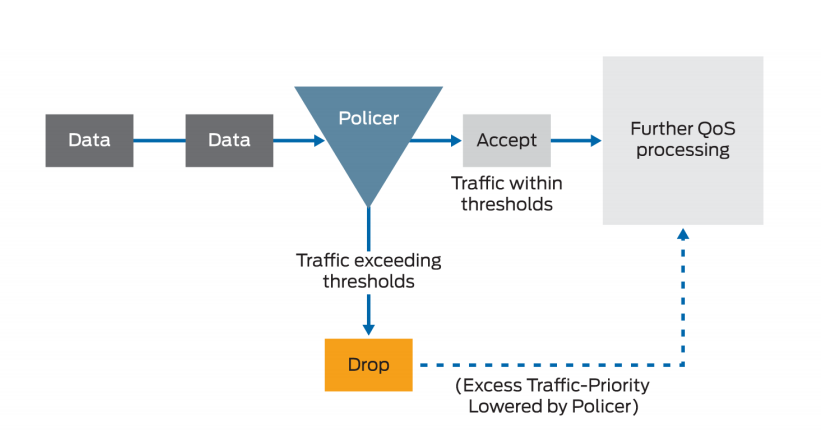
\includegraphics[width=0.5\textwidth]{img/policer.png}}
	\caption{QoS Policers}
	\label{fig:qos01}
\end{figure}
In this project the function of the \textit{policer} will be used intensively.\\
Policers control traffic bursts by ensuring that incoming or outgoing traffic conforms to a configured rate called the bandwidth limit. Policers provide the first line of congestion management by preventing incoming traffic from overloading the network. Figure \ref{fig:qos01} illustrates how policers manage traffic.\\
In many QoS implementations, policers work in conjunction with \textit{metering} and \textit{color marking} tools to increase granularity. Metering measures the traffic arrival rate and assigns different colors to the traffic according to that rate. Metering works by comparing the actual rate of the traffic with the following two configurable values:
\begin{itemize}
  \item Committed information rate (CIR): This is the guaranteed rate.
  \item Peak information rate (PIR): This is te maximum allowed traffic rate.
\end{itemize}
Metering measures the traffic comparing these two values and marks the traffic with colors that identify whether the traffic is \textit{in-contract} or \textit{out-of-contract} as follows:
\begin{itemize}
  \item \textcolor{green}{Green:} Traffic rate is below the CIR and is in-contract.
  \item \textcolor{orange}{Yellow:} Traffic rate falls between the CIR and PIR and is out-of-contract.
  \item \textcolor{red}{Red:} Traffic is above the PIR and is out-of-contract.
\end{itemize}
You can configure whether you want the device to forward the traffic or discard it based on the color.\\
Metering has one input, which is the traffic arrival rate, and it has three possible outputs: \textcolor{green}{green}, \textcolor{orange}{yellow}, or \textcolor{red}{red}.\\ \\
In this project we represent the value of the PIR as a constant defined in our script. The measurements we make on our four sensors cannot reach that value, if they do, the \textit{policer} will discard those values.

\section{Implementation Design}\label{sec:imp}
\subsection{\textbf{ Technology:}}
To achieve the simulation of the \textit{policer}, we will use an \textit{Arduino UNO} with a group of sensors: two temperature sensors and two potentiometers that will give variable values to appreciate the work of the \textit{policer}. The Arduino will process the reading of the sensors and display them in real time on graphs where it will be appreciated when a sensor reaches the PIR.

\subsection{\textbf{ Topology:}}
\begin{figure}[h]
	\centerline{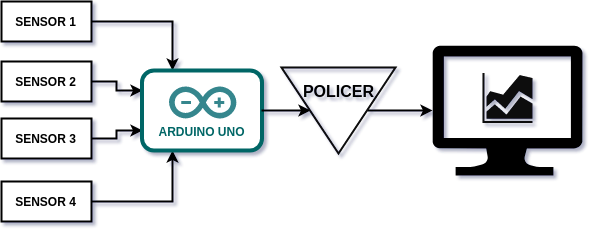
\includegraphics[width=0.4\textwidth]{img/topology01.png}}
	\caption{Topology}
	\label{fig:top01}
\end{figure}
The sensor values are received by the Arduino and processed by a Python script through the serial port. The QoS parameters for metering and coloring are defined in the script. The sensor data is plotted by the same script in real time.\\
\begin{figure}[h]
	\centerline{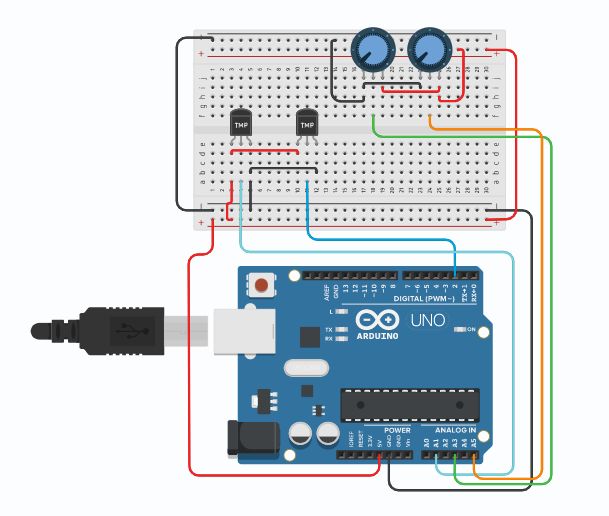
\includegraphics[width=0.5\textwidth]{img/topology.png}}
	\caption{Schematic diagram}
	\label{fig:top02}
\end{figure}

\section{Solution development}\label{sec:met}
The project consists of two parts, the data acquisition part and the processing through the policer.\\
\subsection{Acquisition of data}
Arduino UNO receives signals from temperature sensors and potentiometers through the following script:
\lstinputlisting{script/arduino.ino}
\subsection{Processing}
With the information of the sensor data, the processing and the simulation of the policer are carried out, establishing a PIR value for each signal. A graph will show the values obtained and the effect of the policer.
The python script is as follows:
\lstinputlisting[language = Python]{script/python.py}
\section{Results}
The results were as expected, the graph of the normal values of the sensors with respect to time is observed first. In this case, there are no restrictions and the values are read as they are detected by the sensors.\\
In the second graph, the flag is raised to apply the QoS changes. It is observed that the graph is cut at the PIR points of each sensor, it does not allow values greater than those predefined in the script. In the figure \ref{fig:qos00} you can see the aforementioned.

\begin{figure}[h]
    \begin{subfigure}[h]{0.5\textwidth}
       \centerline{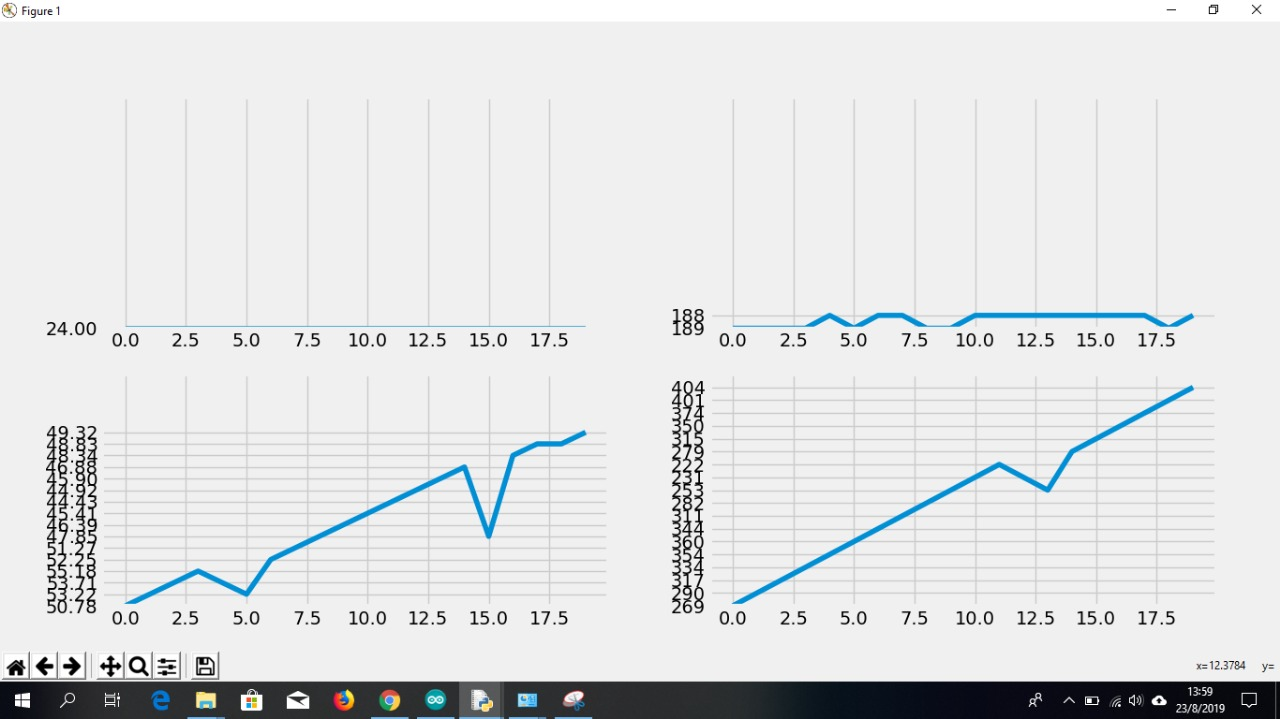
\includegraphics[width=0.85\textwidth]{img/qos.jpeg}}
        \caption{Without QoS}

    \end{subfigure}
    ~ %add desired spacing between images, e. g. ~, \quad, \qquad, \hfill etc.
     \begin{subfigure}[h]{0.5\textwidth}
        \centerline{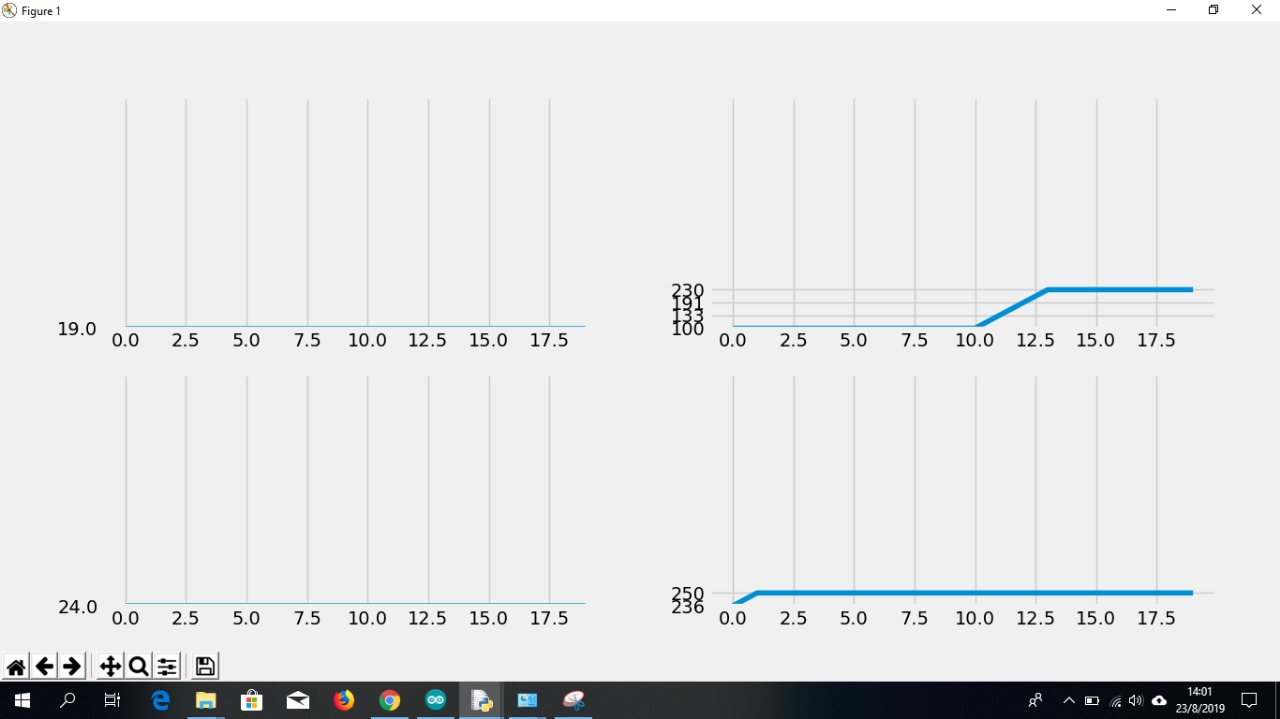
\includegraphics[width=0.85\textwidth]{img/qos2.jpeg}}
        \caption{With QoS}

    \end{subfigure}
    \caption{\textit{Output graphs}}
\label{fig:qos00}
\end{figure}


\section{Conclusions}
\begin{itemize}
	\item The project executes the policer correctly, and its operation is observed in real time.
	\item The developed application can be extended with more functions to be used in any telemetry field.
  \item It is necessary for better application performance to use another device because Arduino presents problems when measuring so much data at the same time, in this way we give scalability to the proposed solution.
\end{itemize}


\begin{thebibliography}{00}
\bibitem{b1}  Juniper Networks, ``Learn About Quality of Services (QoS)'' by Collen Feerick , 2015.

\end{thebibliography}

\end{document}
